%!TEX root = informe.tex
\chapter{Análisis de Ciclo de Vida: fabricación}
% Manual Euroadoquín. Documentos de Malaka.

\section{Introducción}\label{sec:obtenciondedatos}
Los datos de partida que se han utilizado en este análisis han sido proporcionados por Malaka de Prefabricados (Apéndice \ref{apend:datos}). La figura \ref{fig:diagrama_de_flujo} muestra las entradas al sistema, así como los procesos que ocurren durante la fabricación —que serán explicados en las siguientes secciones— y la salida del sistema.

\begin{figure}[!htb]
\centering
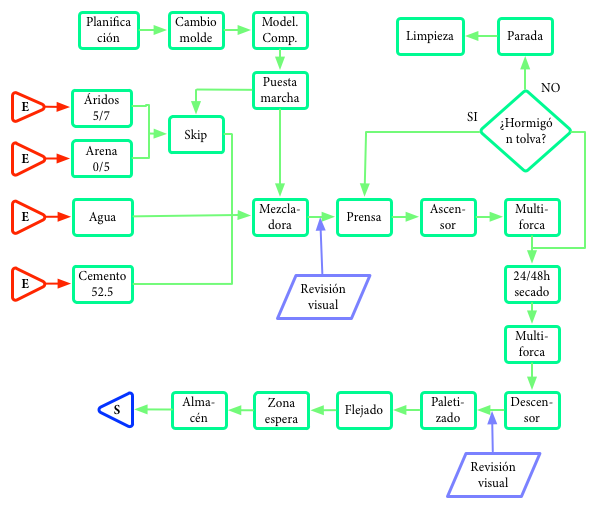
\includegraphics[width=15cm]{diagrama.png}
\caption{Diagrama de flujo de la fabricación de adoquines.}
\label{fig:diagrama_de_flujo}
\end{figure}

El modelo de adoquín ``Holanda 6'' (datos técnicos en Apéndice \ref{apend:catalogo}), es el que mayor demanda de fabricación tiene en la empresa, por lo que se ha dispuesto de mayor número de datos.

\subsection{Unidad funcional}

El motivo de tomar como \textit{Unidad funcional} ``1 \si{m^2} de adoquín'' es debido a que los pedidos y la fabricación se realizan en unidades de superficie y no en cantidad de bloques de adoquín. Cada bandeja fabricada supone exactamente 0.5 \si{m^2} de adoquines modelo ``Holanda 6''. Si se toma como \textit{Unidad funcional} 1 \si{m^2} de adoquín, los cálculos se realizan de forma sencilla para 2 bandejas. Cada adoquín mide 200x100x60 \si{mm} y pesa 3 \si{kg}. Como cada bandeja está formada por 25 adoquines, y son necesarias 2 bandejas para tener 1 \si{m^2}, se tiene un total de 50 adoquines/\si{m^2} (ecuación \ref{eq:masa}). De esta forma:

\begin{gather}
200 mm \times 100 mm \times 25 ud/bandeja \times 2 bandeja = 1 m^2\\
3 kg/ud \times 50 ud/m^2 = 150 kg/m^2 \text{ de masa para adoquín}\label{eq:masa}
\end{gather}

Como es necesario disponer de 150 \si{kg/m^2} de masa para adoquín, se aplican los porcentajes de materias primas sobre la fórmula base para adoquín ``Holanda 6'' para obtener las masas de cada materia prima reflejadas en la tabla \ref{desglosemateriasprimas}.

\begin{table}[!htb]
\centering
\begin{tabular}{lcccc}
\toprule
\multicolumn{5}{c}{Consumo de materias primas por \si{m^2} de adoquín fabricado}\\
\midrule
Materia prima & \% Fórmula & Masa (\si{kg}) & Proced. & Dist. (\si{km})\\
\midrule
Árido tipo 5/7 & 37.75 & 56.63 & Alh. Torre & 8\\
Arena tipo 0/5 & 47.16 & 70.74 & Alh. Torre & 8\\
Cemento Portland 52.5N & 10.06 & 15.09 & Málaga-El Palo & 30\\
Agua & 5.03 & 7.54 & Red & -\\
\bottomrule
\end{tabular}
\caption{Desglose de materias primas por \si{m^2} de adoquín fabricado.}
\label{desglosemateriasprimas}
\end{table}

En el Apéndice \ref{apend:catalogo} también se especifica un diagrama de Gantt de los procesos para una simulación realizada para fabricar 1 \si{m^2} de adoquín, además de los consumos energéticos desglosados.

\section{Modelado de materias primas y procesos}\label{sec:modeladoprocesos}
\subsection{Cemento}
El cemento se transporta a granel en camiones con tanques a presión hasta la fábrica. Allí se almacena en silos provistos de compresores que descargan el material desde el tanque hasta su interior. El compresor es alimentado por electricidad mediante una toma de corriente conectada a la red eléctrica. La descarga del silo es únicamente por gravedad con válvulas dosificadoras de control de caudal (ver tabla \ref{modeladodelcemento}).

Las unidades para el modelado del camión (lorry) vienen expresadas en \si{kg\times km}, mientras que el uso del silo se proporciona en \si{m^3}, dada una densidad media del cemento Portland de 1250 \si{kg/m3} \cite{website:ecoinvent}.

\begin{gather}
15.09 kg \times 30 km = 453 kg\times km\\
15,09 kg / 1250 kg/m^3 = 0.0121 m^3
\end{gather}

El mix eléctrico se obtiene del consumo del compresor del silo proporcional a una cantidad de 15.09 \si{kg}, si la potencia del compresor son 30kW, velocidad de carga del silo es 35 \si{\tonne/h} para un tiempo de llenado de 35 minutos.

\begin{gather}
30 kW \times 1 h \times \frac{35 min}{60 min} = 17.5 kWh = 63 MJ \text{ para 20 toneladas}\\
35 t/h \times \frac{35 min}{60 min} = 20 t \text{ de cemento con el silo cargado}\\
15.09 kg \times \frac{63 MJ}{20 t} = 4.79 kJ
\end{gather}

\begin{table}[!htb]
\centering
\begin{tabular}{p{8cm}rc}
\toprule
\multicolumn{3}{c}{Cemento Portland CEM I 52.5Z gris}\\
\midrule
Materiales/ensamblajes & Cantidad & Unidad\\
\midrule
Portland cement, strength class Z 52.5, at plant/CH U & 15.09 & \si{kg}\\
\midrule
Procesos & Cantidad & Unidad\\
\midrule
Transport, lorry 16-32t, EURO4/RER U & 453 & \si{kg*km}\\
Tower silo, plastic/CH/I U & 0.0121 & \si{m^3}\\
Electricity mix 2013/ES U & 4.79 & \si{kJ}\\
\bottomrule
\end{tabular}
\caption{Modelado del cemento.}
\label{modeladodelcemento}
\end{table}

\subsection{Arena y áridos}
Las arenas y áridos se transportan hasta la planta de fabricación mediante camiones. Actualmente los áridos y la arena ya no se apilan a bajo techados en las explanadas adyacentes a las plantas, sino que el propio transporte rellena las tolvas de forma automática.

El tipo de arena que se utiliza en la planta es 0/5 —granulometría en milímetros de las partículas que forman la arena— no está directamente disponible en SimaPro. En su lugar, se ha optado por tomar el material ``Sand 0/2'' (Arena tipo 0/2), que además de pertenecer a la clasificación general de arena —de 0 a 5 \si{mm}—, la descripción de SimaPro indica que puede utilizarse como árido natural estándar en la industria de la construcción (ver tabla \ref{modeladodelaarena}).

\begin{quote}
Technical purpose of product or process: Standard mineral product used as natural aggregates in the construction industry according to the applied technology.
\end{quote}

Las unidades para el modelado del camión (lorry) vienen expresadas en \si{kg\times km}.

\begin{equation}
70.74 kg \times 8 km = 566 kg\times km
\end{equation}

\begin{table}[!htb]
\centering
\begin{tabular}{p{8cm}rc}
\toprule
\multicolumn{3}{c}{Arena tipo 0/5}\\
\midrule
Materiales/ensamblajes & Cantidad & Unidad\\
\midrule
Sand 0/2, wet and dry quarry, production mix, at plant, undried/RER S & 70.74 & \si{kg}\\
\midrule
Procesos & Cantidad & Unidad\\
\midrule
Transport, lorry 16-32t, EURO4/RER U & 566 & \si{kg*km}\\
\bottomrule
\end{tabular}
\caption{Modelado de la arena.}
\label{modeladodelaarena}
\end{table}

Los áridos utilizados para producir adoquines puede incluir arena, gravilla y piedra de machaqueo si se pretende obtener un producto de peso normal. Si se desea que el adoquín sea más ligero —entre un 20 y un 45 \%— sin mermar sus propiedades estructurales se utilizan materiales como pizarra, arcilla, escoria de altos hornos y cenizas de carbón según su disponibilidad y coste.

El tipo de árido utilizado en planta es de granulometría 5/7 —en milímetros—, catalogado como gravilla. No está directamente disponible en SimaPro, por lo que en su lugar, se ha optado por tomar el material ``Gravel, crushed'' (gravilla de machaqueo) (tabla \ref{modeladodearido}).

Las unidades para el modelado del camión (lorry) vienen expresadas en \si{kg\times km}.

\begin{equation}
56.63 kg \times 8 km = 566 kg\times km
\end{equation}

\begin{table}[!htb]
\centering
\begin{tabular}{p{8cm}rc}
\toprule
\multicolumn{3}{c}{Árido tipo 5/7}\\
\midrule
Materiales/ensamblajes & Cantidad & Unidad\\
\midrule
Gravel, crushed, at mine/CH U & 56.63 & \si{kg}\\
\midrule
Procesos & Cantidad & Unidad\\
\midrule
Transport, lorry 16-32t, EURO4/RER U & 453 & \si{kg*km}\\
\bottomrule
\end{tabular}
\caption{Modelado del árido.}
\label{modeladodearido}
\end{table}


\subsection{Agua}
La mayoría de las plantas tienen una fuente de agua municipal (\textit{tap water}) que proporciona potable perfectamente válida para el uso en la fabricación de hormigón (ver tabla \ref{modeladodelagua}).

\begin{table}[!htb]
\centering
\begin{tabular}{p{8cm}rc}
\toprule
\multicolumn{3}{c}{Agua}\\
\midrule
Materiales/ensamblajes & Cantidad & Unidad\\
\midrule
Tap water, at user/RER U & 7.54 & \si{kg}\\
\bottomrule
\end{tabular}
\caption{Modelado del agua.}
\label{modeladodelagua}
\end{table}

\subsection{Mix eléctrico}

El mix eléctrico es el valor que expresa las emisiones de \ce{CO2} asociadas a la generación de la electricidad que se consume.

Es un indicador de las fuentes energéticas que se emplean para producir electricidad. Cuanto más bajo es el mix, mayor es la contribución de fuentes energéticas bajas en carbono.

Disponer de un mix eléctrico actualizado ayuda a obtener unos resultados más precisos en el Análisis de Ciclo de Vida. La base de datos de \textit{ecoinvent} proporciona un modelo no actualizado para España, sobretodo teniendo en cuenta los últimos avances en adopción de energías renovables en el sector energético español. De esta forma, se ha añadido un nuevo modelo (tabla \ref{modeladomixelectrico}) con las cifras actualizadas al presente año para 1 \si{kWh} \cite{mlgceballos}.

\begin{table}[!htb]
\centering
\begin{tabular}{p{8cm}rc}
\toprule
\multicolumn{3}{c}{Electricity mix 2013/ES U}\\
\midrule
Materiales/combustibles & Cantidad & Unidad\\
\midrule
Electricity, hard coal, at power plant/ES U & 0.0596 & \si{kWh}\\
Electricity, lignite, at power plant/ES U & 0.0268 & \si{kWh}\\
Electricity, oil, at power plant/ES U & 0.0527 & \si{kWh}\\
Electricity, natural gas, at power plant/ES U & 0.3025 & \si{kWh}\\
Electricity, industrial gas, at power plant/ES U & 0.0147 & \si{kWh}\\
Electricity, hydropower, at power plant/ES U & 0.131 & \si{kWh}\\
Electricity, hydropower, at pumped storage power plant/ES U & 0.020 & \si{kWh}\\
Electricity, nuclear, at power plant/UCTE U & 0.205 & \si{kWh}\\
Electricity, production mix photovoltaic, at plant/ES U & 0.024 & \si{kWh}\\
Electricity, at wind power plant/RER U & 0.1454 & \si{kWh}\\
Electricity, at cogen with biogas engine, allocation exergy/CH U & 0.0146 & \si{kWh}\\
Electricity, production mix FR/FR U & 0.0056 & \si{kWh}\\
\bottomrule
\end{tabular}
\caption{Modelado del mix eléctrico español en 2013.}
\label{modeladomixelectrico}
\end{table}

\subsection{Dosificador de arena y áridos}

El sistema de control central manda una señal a los dosificadores para que viertan la cantidad ordenada por el programa principal de fabricación. Dichos dosificadores consisten en una especie de tolva con forma de embudo con un cierre controlado por el sistema.

No existe un modelo de referencia en SimaPro para este tipo de dosificadores —\textit{feed hopper}, en inglés—, por lo que se ha simplificado un modelo válido \cite{woodpellet}. Se le ha añadido la parte de mix eléctrico de los datos del fabricante (Apéndice \ref{apend:datos}). El dosificador del cemento y del agua están incluidos en su propio modelo (silo y abastecimiento de la red respectivamente).

\begin{table}[!htb]
\centering
\begin{tabular}{p{8cm}rc}
\toprule
\multicolumn{3}{c}{Dosificadores para arena y áridos}\\
\midrule
Materiales/combustibles & Cantidad & Unidad\\
\midrule
Steel, low-alloyed, at plant/RER U & 47 & \si{kg}\\
\midrule
Electricidad/calor & Cantidad & Unidad\\
\midrule
Electricity mix 2013/ES U & 0.0021 & \si{MJ}\\
\bottomrule
\end{tabular}
\caption{Modelado de los dosificadores para arena y áridos.}
\label{modeladodedosificadores}
\end{table}

\subsection{Cintas transportadoras de áridos y cemento}

Las tolvas descargan la cantidad programada de materia prima sobre dos cintas transportadoras —una para áridos y arena, otra para cemento— con básculas de pesaje incorporadas que se comunican con el sistema de control y cortan el flujo de descarga.

La cinta de áridos descarga sobre un skip que eleva los materiales hasta una mezcladora. La cinta de cemento descarga directamente sobre la mezcladora.

Las distancias están medidas sobre planos (Apéndice \ref{apend:planos}), y los consumos se han obtenido de los ensayos en fábrica a partir de la potencia de la cinta transportadora y el tiempo de funcionamiento (Potencia=Energía/Tiempo).

\begin{table}[!htb]
\centering
\begin{tabular}{p{8cm}rc}
\toprule
\multicolumn{3}{c}{Cinta transportadora para arena y áridos}\\
\midrule
Materiales/combustibles & Cantidad & Unidad\\
\midrule
Conveyor belt, at plant/RER/I U & 14.6 & \si{m}\\
\midrule
Electricidad/calor & Cantidad & Unidad\\
\midrule
Electricity mix 2013/ES U & 0.1827 & \si{MJ}\\
\bottomrule
\end{tabular}
\caption{Modelado de la cinta transportadora para arena y áridos.}
\label{modeladodecintaarena}
\end{table}

\begin{table}[!htb]
\centering
\begin{tabular}{p{8cm}rc}
\toprule
\multicolumn{3}{c}{Cinta transportadora para cemento}\\
\midrule
Materiales/combustibles & Cantidad & Unidad\\
\midrule
Conveyor belt, at plant/RER/I U & 7.3 & \si{m}\\
\midrule
Electricidad/calor & Cantidad & Unidad\\
\midrule
Electricity mix 2013/ES U & 0.0975 & \si{MJ}\\
\bottomrule
\end{tabular}
\caption{Modelado de la cinta transportadora para cemento.}
\label{modeladodecintacemento}
\end{table}

\subsection{Skip y mezcladora}

Para asegurar la consistencia del lote el agua se añade mediante un sistema electrónico de control que dosifica el caudal. En el caso de que haya otros aditivos, tales como acelerantes o colorantes, es en este momento cuando se incorporan a la mezcla. Cuando se termina de añadir el agua se produce el mezclado creando hormigón fresco.

La base de datos \textit{ecoinvent} proporciona un modelo para el mezclado del hormigón, ``Paster mixing'' en el que se introduce la masa de la mezcla, 150 \si{kg} y al que se le añade la parte de mix eléctrico de los datos del fabricante (Apéndice \ref{apend:datos}).

\begin{table}[!htb]
\centering
\begin{tabular}{p{8cm}rc}
\toprule
\multicolumn{3}{c}{Skip y mezcladora}\\
\midrule
Materiales/combustibles & Cantidad & Unidad\\
\midrule
Plaster mixing/CH U & 150 & \si{kg}\\
\midrule
Electricidad/calor & Cantidad & Unidad\\
\midrule
Electricity mix 2013/ES U & 1.71 & \si{MJ}\\
\bottomrule
\end{tabular}
\caption{Modelado del skip y la mezcladora.}
\label{modeladoskip}
\end{table}

\subsection{Cinta transportadora para hormigón}

El hormigón sale de la mezcladora mediante una cinta transportadora que contiene otra báscula de pesaje y se dirige hacia la tolva de hormigón que se encuentra en lo alto de la prensa.

La base de datos \textit{ecoinvent} proporciona un modelo para la cinta transportadora, ``Conveyor belt'' en el que se introduce la distancia de recorrido, 12.1 \si{m}, y al que se le añade la parte de mix eléctrico de los datos del fabricante (Apéndice \ref{apend:datos}).

\begin{table}[!htb]
\centering
\begin{tabular}{p{8cm}rc}
\toprule
\multicolumn{3}{c}{Cinta transportadora para hormigón}\\
\midrule
Materiales/combustibles & Cantidad & Unidad\\
\midrule
Conveyor belt, at plant/RER/I U & 12.1 & \si{m}\\
\midrule
Electricidad/calor & Cantidad & Unidad\\
\midrule
Electricity mix 2013/ES U & 0.088 & \si{MJ}\\
\bottomrule
\end{tabular}
\caption{Modelado de la cinta transportadora para hormigón.}
\label{modeladodecintahormigon}
\end{table}

\subsection{Tolva para hormigón}

La tolva de hormigón se encarga de dosificar el hormigón en el molde de la prensa. No existe un modelo de referencia en SimaPro para tolvas —\textit{hopper}, en inglés—, por lo que se ha simplificado un modelo válido \cite{foodnottrash}. Se le ha añadido la parte de mix eléctrico de los datos del fabricante (Apéndice \ref{apend:datos}).

\begin{table}[!htb]
\centering
\begin{tabular}{p{8cm}rc}
\toprule
\multicolumn{3}{c}{Tolva para hormigón}\\
\midrule
Materiales/combustibles & Cantidad & Unidad\\
\midrule
Steel, low-alloyed, at plant/RER U & 470 & \si{kg}\\
\midrule
Electricidad/calor & Cantidad & Unidad\\
\midrule
Electricity mix 2013/ES U & 0.0161 & \si{MJ}\\
\bottomrule
\end{tabular}
\caption{Modelado de la tolva para hormigón.}
\label{modeladotolvahormigon}
\end{table}

\subsection{Vibrocompresión}

La tolva dosifica el hormigón fresco, que cae en los moldes para adoquines. Los moldes tienen una longevidad muy alta —aproximadamente un millón de ciclos de prensado— y su durabilidad depende de las propiedades abrasivas de los áridos utilizados.

El molde se compone de dos partes: la parte donde se inyecta el hormigón (hembra) y la parte que se coloca encima para dar forma (macho). La prensa tiene incorporado un carro alimentador encargado de proporcionar la parte hembra. Se inyecta el hormigón en el molde hembra, el molde macho baja con la prensa y el hormigón es compactado y cimentado usando un sistema combinado de presión y vibración. Cada molde puede producir 25 adoquines de 200x100x60\si{\milli\meter}, lo que proporciona a una superficie adoquinada de 0.5\si{\square\meter}. Los adoquines son moldeados de una sola pieza y extraidos del molde inmediatamente después de la vibro-compresión sobre una bandeja de madera.

SimaPro no proporciona un modelo para prensas de cemento. Estudiando las similitudes entre una planta de hormigón —\textit{concrete plant}— y la planta objeto de este proyecto, se puede aproximar un modelo de la prensa basado en la maquinaria del primero \cite{buildingproducts}. La aproximación ``Industrial machine, heavy, unspecified, at plant'' pide la masa de la máquina industrial no específica que realiza el proceso. De acuerdo al fabricante, ese dato es de 1380 \si{kg}, al que se le ha añadido la parte de mix eléctrico también proporcionado por el fabricante (Apéndice \ref{apend:datos}).

\begin{table}[!htb]
\centering
\begin{tabular}{p{8cm}rc}
\toprule
\multicolumn{3}{c}{Prensado}\\
\midrule
Materiales/combustibles & Cantidad & Unidad\\
\midrule
Industrial machine, heavy, unspecified, at plant/RER/I U & 9000 & \si{kg}\\
\midrule
Electricidad/calor & Cantidad & Unidad\\
\midrule
Electricity mix 2013/ES U & 0.437 & \si{MJ}\\
\bottomrule
\end{tabular}
\caption{Modelado del prensado.}
\label{modeladoprensado}
\end{table}

\subsection{Cinta transportadora para piezas frescas}

La bandeja con las piezas frescas es trasladada sobre un transportador de rodillos hasta un ascensor.

SimaPro no proporciona un modelo para este tipo de transportador. Estudiando las similitudes entre un transportador de rodillos y una cinta transportadora se puede aproximar un modelo propio basado en que la principal diferencia es la falta de una banda de rodadura (tabla \ref{modeladotransportadorrodillos}).

\begin{table}[!htb]
\centering
\begin{tabular}{p{8cm}rc}
\toprule
\multicolumn{3}{c}{Transportadora de rodillos para piezas frescas}\\
\midrule
Materiales/combustibles & Cantidad & Unidad\\
\midrule
Concrete, sole plate and foundation, at plant/CH U & 0.01 & \si{m^3}\\
Section bar rolling, steel/RER U & 500 & \si{kg}\\
Steel, low-alloyed, at plant/RER U & 530 & \si{kg}\\
Transport, lorry >16t, fleet average/RER U & 55.5 & \si{\tonne\times km}\\
Wire drawing, steel/RER U & 29.6 & \si{kg}\\
\midrule
Residuos y emisiones para tratamiento & Cantidad & Unidad\\
\midrule
Disposal, building, reinforced concrete, to final disposal/CH U & 23 & \si{kg}\\
Disposal, steel, 0\% water, to municipal incineration/CH U & 29.6 & \si{kg}\\
\bottomrule
\end{tabular}
\caption{Modelado de 1 metro de transportador de rodillos.}
\label{modeladotransportadorrodillos}
\end{table}

La aproximación ``Roller conveyor, at plant'' pide como parámetro la distancia de recorrido, 6.8 \si{m}, al que se le ha añadido la parte de mix eléctrico también proporcionado por el fabricante (Apéndice \ref{apend:datos}).

\begin{table}[!htb]
\centering
\begin{tabular}{p{8cm}rc}
\toprule
\multicolumn{3}{c}{Transportadora de rodillos para piezas frescas}\\
\midrule
Materiales/combustibles & Cantidad & Unidad\\
\midrule
Conveyor belt, at plant/RER/I U & 6.8 & \si{m}\\
\midrule
Electricidad/calor & Cantidad & Unidad\\
\midrule
Electricity mix 2013/ES U & 0.077 & \si{MJ}\\
\bottomrule
\end{tabular}
\caption{Modelado del transportador de rodillos para piezas frescas.}
\label{modeladotransportadorpiezas}
\end{table}

\subsection{Ascensor}

Este ascensor tiene diez alturas, de forma que cada vez que recibe una bandeja con adoquines frescos, la bandeja anterior sube una altura y monta la siguiente. El ascensor se encarga de alimentar un carro multiforca de diez alturas.

SimaPro no proporciona un modelo para un ascensor de estas características, por lo que se ha obtado por un elemento genérico que sí esté en la base de datos de \textit{ecoinvent} como ``Industrial machine, heavy, unspecified, at plant'' que pide la masa de la máquina industrial no específica que realiza el proceso. De acuerdo al fabricante, ese dato es de 320 \si{kg}, al que se le ha añadido la parte de mix eléctrico también proporcionado por el fabricante (Apéndice \ref{apend:datos}).

\begin{table}[!htb]
\centering
\begin{tabular}{p{8cm}rc}
\toprule
\multicolumn{3}{c}{Ascensor}\\
\midrule
Materiales/combustibles & Cantidad & Unidad\\
\midrule
Industrial machine, heavy, unspecified, at plant/RER/I U & 320 & \si{kg}\\
\midrule
Electricidad/calor & Cantidad & Unidad\\
\midrule
Electricity mix 2013/ES U & 0.126 & \si{MJ}\\
\bottomrule
\end{tabular}
\caption{Modelado del ascensor.}
\label{modeladodelascensor}
\end{table}

\subsection{Multiforca}
Cuando las diez alturas está ocupadas se cargan en un carro multiforca —\textit{rack transporter}, en inglés— automatizado que transporta las piezas hasta un secadero.

Las piezas permanecen en el secadero curándose a temperatura ambiente entre 24 y 48 horas.

Una vez transcurrido el tiempo de curado, los adoquines están secos y listos para ser recogidos por otro carro multiforca automatizado que recoge las bandejas y las lleva a un descensor.

SimaPro tampoco proporciona un modelo para un carro multiforca, por lo que también se ha obtado por un elemento genérico que sí esté en la base de datos de \textit{ecoinvent} como ``Industrial machine, heavy, unspecified, at plant'' que pide la masa de la máquina industrial no específica que realiza el proceso. De acuerdo al fabricante, un carro multiforca se compone de un tres partes: transportador de forca (rackveyor), rodadura (crawler) y vehículo (transfer car), sumando en total 7500 \si{kg}, a lo que se le ha añadido la parte de mix eléctrico también proporcionado por el fabricante (Apéndice \ref{apend:datos}).

\begin{table}[!htb]
\centering
\begin{tabular}{p{8cm}rc}
\toprule
\multicolumn{3}{c}{Multiforca}\\
\midrule
Materiales/combustibles & Cantidad & Unidad\\
\midrule
Industrial machine, heavy, unspecified, at plant/RER/I U & 7500 & \si{kg}\\
\midrule
Electricidad/calor & Cantidad & Unidad\\
\midrule
Electricity mix 2013/ES U & 0.516 & \si{MJ}\\
\bottomrule
\end{tabular}
\caption{Modelado de la multiforca.}
\label{modeladomultiforca}
\end{table}

\subsection{Descensor}
El descensor coloca las bandejas con los adoquines secos en un transportador de rodillos. Su modelado es el mismo que el del ascensor.

\begin{table}[!htb]
\centering
\begin{tabular}{p{8cm}rc}
\toprule
\multicolumn{3}{c}{Descensor}\\
\midrule
Materiales/combustibles & Cantidad & Unidad\\
\midrule
Industrial machine, heavy, unspecified, at plant/RER/I U & 320 & \si{kg}\\
\midrule
Electricidad/calor & Cantidad & Unidad\\
\midrule
Electricity mix 2013/ES U & 0.126 & \si{MJ}\\
\bottomrule
\end{tabular}
\caption{Modelado del descensor.}
\label{modeladodeldescensor}
\end{table}

\subsection{Transporte de bandejas hasta paletizadora}
El transportador de rodillos lleva las bandejas hasta una paletizadora para hacer bloques de hasta cinco alturas. Se ha vuelto a utilizar el modelado de la tabla \ref{modeladotransportadorrodillos}, introduciendo los 6.88 \si{m} de recorrido entre el origen y el destino, a lo que se le ha añadido la parte de mix eléctrico también proporcionado por el fabricante (Apéndice \ref{apend:datos}).

\begin{table}[!htb]
\centering
\begin{tabular}{p{8cm}rc}
\toprule
\multicolumn{3}{c}{Transporte de bandejas hasta paletizadora}\\
\midrule
\multicolumn{2}{c}{Materiales/combustibles}\\
\cmidrule(r){1-2}
Descripción & Cantidad & Unidad\\
\midrule
Roller conveyor, at plant/RER/I U & 6.88 & \si{m}\\
\midrule
\multicolumn{2}{c}{Electricidad/calor}\\
\cmidrule(r){1-2}
Descripción & Cantidad & Unidad\\
\midrule
Electricity mix 2013/ES U & 0.021 & \si{MJ}\\
\bottomrule
\end{tabular}
\caption{Modelado del transporte de bandejas hasta paletizadora.}
\label{modeladobandejaspalet}
\end{table}

\subsection{Paletizado y flejado}

La paletizadora dispone los bloques de adoquín sobre un pallet para su posterior almacenaje y transporte. De esta forma se consigue una mayor uniformidad y facilidad de manipulación de la carga, ahorrando espacio y rentabilizando los tiempos de carga—descarga y manipulación.

La paletizadora impulsa el pallet hasta la flejadora que aplica varias lazadas de flejes para evitar que los adoquines se desprendan del conjunto.

El proceso de SimaPro ``Packing, clay products'' abarca ambos procesos en un único modelo, en el que se introduce la masa de la carga, 150 \si{km}, a lo que se le ha añadido la parte de mix eléctrico proporcionado por el fabricante (Apéndice \ref{apend:datos}).

\begin{table}[!htb]
\centering
\begin{tabular}{p{8cm}rc}
\toprule
\multicolumn{3}{c}{Flejado y paletizado}\\
\midrule
Materiales/combustibles & Cantidad & Unidad\\
\midrule
Packing, clay products/CH U & 150 & \si{kg}\\
\midrule
Electricidad/calor & Cantidad & Unidad\\
\midrule
Electricity mix 2013/ES U & 0.065 & \si{MJ}\\
\bottomrule
\end{tabular}
\caption{Modelado del flejado y paletizado.}
\label{modeladodelflejadoypaletizado}
\end{table}

\begin{table}[!htb]
\centering
\begin{tabular}{p{8cm}rc}
\toprule
\multicolumn{3}{c}{Transporte de pallets hasta flejadora}\\
\midrule
Materiales/combustibles & Cantidad & Unidad\\
\midrule
Roller conveyor, at plant/RER/I U & 3.1 & \si{m}\\
\midrule
Electricidad/calor & Cantidad & Unidad\\
\midrule
Electricity mix 2013/ES U & 0.021 & \si{MJ}\\
\bottomrule
\end{tabular}
\caption{Modelado del transporte de pallets hasta flejadora.}
\label{modeladopalletsflejadora}
\end{table}

\subsection{Transporte de pallets flejados hasta zona de recogida}

La flejadora descansa los conjuntos paletizados sobre un un transportador de rodillos para ser posteriormente llevados a almacén.

\begin{table}[!htb]
\centering
\begin{tabular}{p{8cm}rc}
\toprule
\multicolumn{3}{c}{Transporte de pallets flejados hasta zona de recogida}\\
\midrule
Materiales/combustibles & Cantidad & Unidad\\
\midrule
Roller conveyor, at plant/RER/I U & 39.1 & \si{m}\\
\midrule
Electricidad/calor & Cantidad & Unidad\\
\midrule
Electricity mix 2013/ES U & 0.0315 & \si{MJ}\\
\bottomrule
\end{tabular}
\caption{Modelado del transporte de pallets flejados hasta zona de recogida.}
\label{modeladopalletsrecogida}
\end{table}

\subsection{Transporte de pallets hasta almacén}
Finalmente, un toro de almacén (forklift truck) transporta cada pallet de adoquines a la zona de almacenaje, a la espera de que los pedidos salgan de almacén.

SimaPro no incorpora en ninguna de sus bases de datos un modelo aproximado de un toro, generando el modelo de la tabla \ref{modeladoforklift}. El modelo comprende el habitáculo, horquilla, motor, batería, neumáticos y su parte proporcional de trabajo de mecanizado y ensamblado \cite{ecocosts}.

\begin{table}[!htb]
\centering
\begin{tabular}{p{8cm}rc}
\toprule
\multicolumn{3}{c}{Forklift truck}\\
\midrule
Materiales/combustibles & Cantidad & Unidad\\
\midrule
Steel, low-alloyed, at plant/RER U & 2250 & \si{kg}\\
Lead, primary, at plant/GLO U & 1200 & \si{kg}\\
Sulfuric acid, at plant/kg/RNA & 2800 & \si{kg}\\
Acrylonitrile-butadiene-styrene copolymer, ABS, at plant/RER U & 90 & \si{kg}\\
Copper, at regional storage/RER U & 50 & \si{kg}\\
Turning, steel, conventional, primarily roughing/RER S & 1000 & \si{kg}\\
Drilling, CNC, steel/RER U & 1250 & \si{kg}\\
Copper wire, technology mix, consumption mix, at plant, cross section 1 mm² EU-15 S & 50 & \si{kg}\\
\bottomrule
\end{tabular}
\caption{Modelado de un toro de almacén (forklift truck).}
\label{modeladoforklift}
\end{table}

Al igual que no incluye un modelo de toro, tampoco incluye el transporte mediante un toro de almacén, por lo que se ha establecido un modelado basado en el de un furgón de carga de menos de 3.5 \si{\tonne} para añadir las partes proporcionales de uso del toro, mantenimiento, asfalto y costes de operación (tabla \ref{modeladotransporteforklift}).

\begin{table}[!htb]
\centering
\begin{tabular}{p{8cm}rc}
\toprule
\multicolumn{3}{c}{Transport, forklift truck}\\
\midrule
Materiales/combustibles & Cantidad & Unidad\\
\midrule
Operation, van < 3,5t/RER U & 5.3015 & \si{km}\\
Forklift truck & 0.000024098 & p\\
Maintenance, van < 3.5t/RER/I U & 0.000024098 & p\\
Road/CH/I U & 0.0067419 & \si{my}\\
Operation, maintenance, road/CH/I U & 0.0062138 & \si{my}\\
\midrule
Residuos y emisiones & Cantidad & Unidad\\
Disposal, van < 3.5t/CH/I U & 0.000024098 & p\\
Disposal, road/RER/I U & 0.0067419 & \si{my}\\
\midrule
\bottomrule
\end{tabular}
\caption{Modelado del transporte con toro de almacén.}
\label{modeladotransporteforklift}
\end{table}

De esta forma, el modelado del transporte con el toro hasta el almacén se genera introduciendo las toneladas por kilómetro que se transportan (tabla \ref{modeladotransportetorito}).

\begin{table}[!htb]
\centering
\begin{tabular}{p{8cm}rc}
\toprule
\multicolumn{3}{c}{Transporte de pallets con torito hasta almacén}\\
\midrule
Materiales/combustibles & Cantidad & Unidad\\
\midrule
Transport, forklift truck/RER U & 0.0132 & \si{\tonne\times km}\\
\bottomrule
\end{tabular}
\caption{Modelado del transporte de pallets con torito hasta almacén.}
\label{modeladotransportetorito}
\end{table}

\subsection{Control informatizado}

Todo el sistema está centralizado en dos ordenadores que cargan los programas de funcionamiento situados en una cabina supervisada por un operario.

\begin{table}[!htb]
\centering
\begin{tabular}{p{8cm}rc}
\toprule
\multicolumn{3}{c}{Control informatizado}\\
\midrule
\multicolumn{2}{c}{Materiales/combustibles}\\
\cmidrule(r){1-2}
Descripción & Cantidad & Unidad\\
\midrule
Desktop computer, without screen, at plant/GLO U & 2 & p\\
Keyboard, standard version, at plant/GLO U & 2 & p\\
LCD flat screen, 17 inches, at plant/GLO U & 2 & p\\
Mouse device, optical, with cable, at plant/GLO U & 2 & p\\
Network access devices, internet, at user/CH/I U & 2 & p\\
Router, IP network, at server/CH/I U & 1 & p\\
Power supply unit, at plant/CN U & 2 & p\\
\midrule
\multicolumn{2}{c}{Electricidad/calor}\\
\cmidrule(r){1-2}
Descripción & Cantidad & Unidad\\
\midrule
Electricity mix 2013/ES U & 0.486 & \si{MJ}\\
\bottomrule
\end{tabular}
\caption{Modelado del control informatizado.}
\label{modeladodecontrol}
\end{table}


\subsection{Iluminación}

La iluminación del recinto se compone principalmente de 60 tubos fluorescentes de 40 \si{W}. Debido a que SimaPro no tiene modelados tubos CFL, se ha añadido un modelo a la base de datos \cite{cflbulb}.

\begin{table}[!htb]
\centering
\begin{tabular}{p{8cm}rc}
\toprule
\multicolumn{3}{c}{Iluminación}\\
\midrule
Materiales/combustibles & Cantidad & Unidad\\
\midrule
CFL Bulb 40W & 60 & p\\
\multicolumn{2}{c}{Desglose para 1 p. CFL Bulb 40W}\\
\cmidrule(r){1-2}
Aluminium alloy, AlMg3, at plant/RER U & 7.09 & \si{g}\\
Oriented polypropylene film E & 4.25 & \si{g}\\
Iron-nickel-chromium alloy, at plant/RER U & 6.27 & \si{g}\\
Copper wire, technology mix, consumption mix, at plant, cross section 1 \si{mm^2} EU-15 S & 4.25 & \si{g}\\
41 Plastics basic, virgin, EU27 & 1.42 & \si{g}\\
Integrated circuit, IC, logic type, at plant/GLO U & 1.42 & \si{g}\\
\midrule
Electricidad/calor & Cantidad & Unidad\\
\midrule
Electricity mix 2013/ES U & 0.972 & \si{MJ}\\
\bottomrule
\end{tabular}
\caption{Modelado de la iluminación.}
\label{modeladodeiluminacion}
\end{table}

\subsection{Limpieza de la mezcladora y molde}

Una vez finalizada la producción se procede a la limpieza de la mezcladora y el molde con agua y vaciando el contenido (tabla \ref{modeladolimpiezamezcladora}).

\begin{table}[!htb]
\centering
\begin{tabular}{p{8cm}rc}
\toprule
\multicolumn{3}{c}{Limpieza de la mezcladora y molde}\\
\midrule
Materiales/combustibles & Cantidad & Unidad\\
\midrule
Tap water, at user/RER/I U & 100 & \si{kg}\\
\bottomrule
\end{tabular}
\caption{Modelado la limpieza de la mezcladora y molde.}
\label{modeladolimpiezamezcladora}
\end{table}

\section{Modelado completo}

Los modelos de los procesos explicados en la sección \ref{sec:modeladoprocesos} han sido introducidos en SimaPro para crear un modelo completo que represente la fabricación de un metro cuadrado de adoquín modelo Holanda 6.

Aunque la mayoría de los procesos sólo ocurren una única vez, hay varios procesos que necesitan funcionar dos veces, debido a que son dos bandejas las que hay que preparar para fabricar el metro cuadrado (ver sección \ref{sec:obtenciondedatos}) o bien, como en el caso de la multiforca, porque hay una ida y una vuelta hacia la zona de curación. El listado completo de procesos se muestra en la tabla \ref{modeladocompleto}.

\begin{table}[!htb]
\centering
\begin{tabular}{p{8cm}rc}
\toprule
\multicolumn{3}{c}{Fabricación 1 \si{m^2} adoquín Holanda 6}\\
\midrule
Materiales/ensamblajes & Cantidad & Unidad\\
\midrule
Agua & 1 & p\\
Arena tipo 0/5 & 1 & p\\
Árido tipo 5/7 & 1 & p\\
\midrule
Procesos & Cantidad & Unidad\\
\midrule
Dosificador de arena & 1 & p\\
Dosificador de áridos & 1 & p\\
Cinta transp. para arena y áridos & 1 & p\\
Cinta transp. para cemento & 1 & p\\
Skip+mezcladora & 1 & p\\
Cinta transp. para hormigón & 1 & p\\
Tolva para hormigón & 2 & p\\
Prensado & 2 & p\\
Transportador de rodillos para piezas frescas & 2 & p\\
Ascensor & 1 & p\\
Multiforca & 2 & p\\
Descensor & 1 & p\\
Transporte de bandejas hasta paletiz. & 1 & p\\
Paletizado+flejado & 1 & p\\
Transporte de pallets hasta flejadora & 1 & p\\
Transporte de pallets flejados hasta zona de recogida & 1 & p\\
Transporte de pallets con torito hasta almacén & 1 & p\\
Control informatizado & 1 & p\\
Iluminación & 1 & p\\
\bottomrule
\end{tabular}
\caption{Modelado completo de la fabricación.}
\label{modeladocompleto}
\end{table}

\section{Resultados}

Una vez creado el modelo completo del proceso de fabricación, SimaPro genera un análisis de los datos introducidos. El método de análisis elegido es \textit{ReCiPe Endpoint (H) V1.06 / Europe ReCipe H/A}, previamente explicado en la sección \ref{sec:recipe}.

\begin{figure}[!htb]
\centering
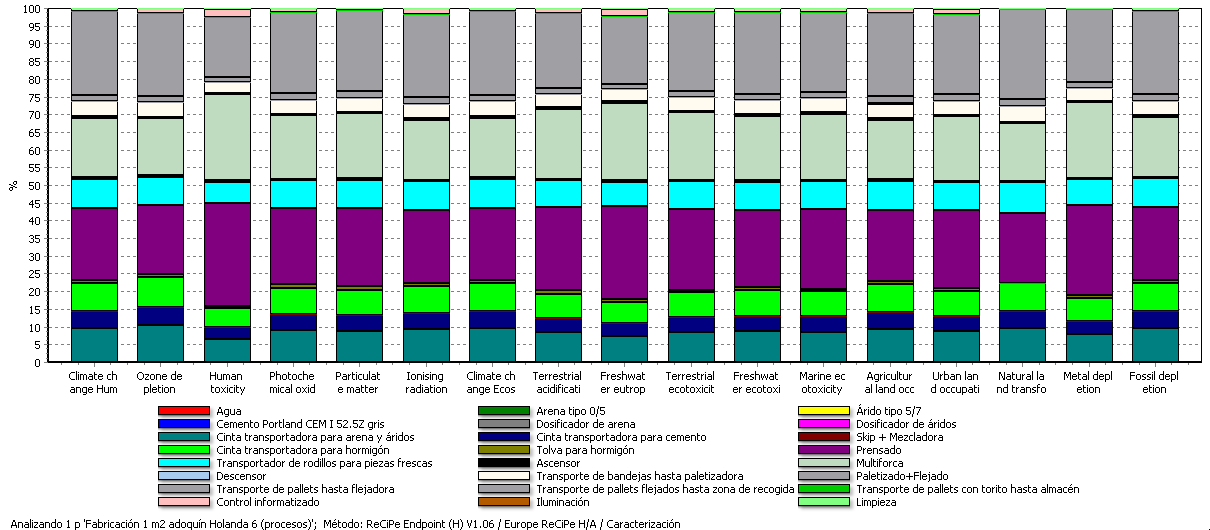
\includegraphics[angle=90,height=19cm]{fabricacion_caracterizacion.png}
\caption{Caracterización del análisis de fabricación de 1 \si{m^2} de adoquín.}
\label{fig:caracterizacionfabricacion}
\end{figure}

\begin{figure}[!htb]
\centering
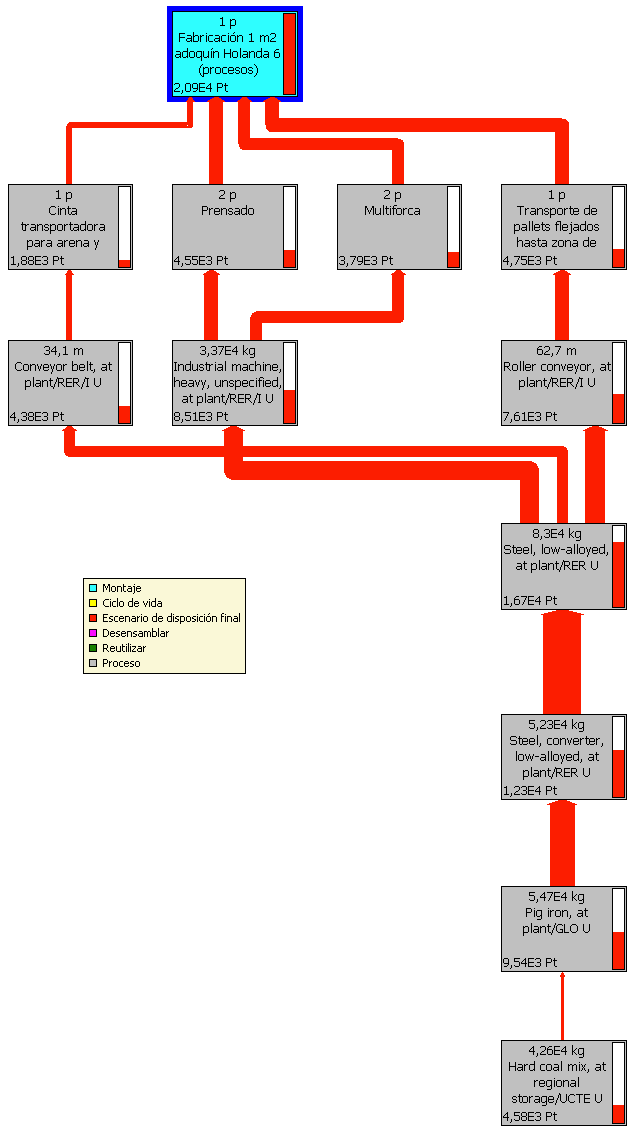
\includegraphics[height=19cm]{fabricacion_red.png}
\caption{Red del análisis de fabricación de 1 \si{m^2} de adoquín.}
\label{fig:redfabricacion}
\end{figure}
